\documentclass[12,a4paper]{article}

\usepackage{graphicx}
\usepackage{float}
\usepackage{caption}
\usepackage{subcaption}
\usepackage{amsmath}
\usepackage{listings}
\usepackage{color}

\definecolor{dkgreen}{rgb}{0,0.6,0}
\definecolor{gray}{rgb}{0.5,0.5,0.5}
\definecolor{mauve}{rgb}{0.58,0,0.82}

\lstset{frame=tb,
  language= C,
  aboveskip=3mm,
  belowskip=3mm,
  showstringspaces=false,
  columns=flexible,
  basicstyle={\small\ttfamily},
  numbers=none,
  numberstyle=\tiny\color{gray},
  keywordstyle=\color{blue},
  commentstyle=\color{dkgreen},
  stringstyle=\color{mauve},
  breaklines=true,
  breakatwhitespace=true,
  tabsize=3
}

\title{High Performance Computing}
\date{\today}
\author{Amarnath Karthi  201501005 \\ Chahak Mehta  201501422}

\setlength{\parindent}{0em}

\makeatletter
\begin{document}
    \begin{titlepage}
	\centering
	{\scshape\LARGE CS-301 \par}
	\vspace{0.1cm}
	{\huge \@title \par}
	\vspace{0.5cm}
	{\Large Assignment 2\par}
	\vspace{10cm}
	\Large Amarnath Karthi          201501005\\
	\Large Chahak Mehta             201501422\\
	\vspace{5cm}
	{\large \@date\par}
\end{titlepage}
    
    
    \section{Hardware Details}
    \begin{table}[H]
        \centering
        \begin{tabular}{c|c}
            \textbf{Parameter} & \textbf{Value} \\\\
            CPU model & Intel Core i5-4590 3.30 GHz \\
            Number of Cores & 4 \\
            L1d Cache & 32 kB \\
            L1i Cache & 32 kB \\
            L2 Cache & 256 kB \\
            L3 Cache & 6144 kB \\
            Compiler & gcc \\
        \end{tabular}
    \end{table}
    
    \section{Problem Statement}
    \textbf{
        Write and analyze serial code and parallel code for the following using OpenMP.
        \begin{enumerate}
            \item Integration of a function using trapezoidal rule. Verify your code by using it to calculate the value of $\pi$.
            \item Calculation of $\pi$ using series.
            \item Summation of two vectors
        \end{enumerate}
    }
    
    \section{Solution}
    \subsection{Integration using trapezoidal rule}
    \subsubsection{Theory}
    We use the following formula to compute the value of $\pi$ :
    \begin{equation}
        \int_{0}^{1} \frac{4}{1+x^2} dx
    \end{equation}
    
    \subsubsection{Approach}
    For the serial code, we use simple numerical integration over 0 to 1. For parallel implementation, we simply run numerical integration over 4 equal ranges of length 0.25 between 0 and 1 over 4 parallel threads. We add each partial sum to the global sum, taking care that the global addition takes place under the \textbf{critical} section.\newpage
    \subsubsection{Results and Observations}
    
    \begin{figure}[H]
        \centering
        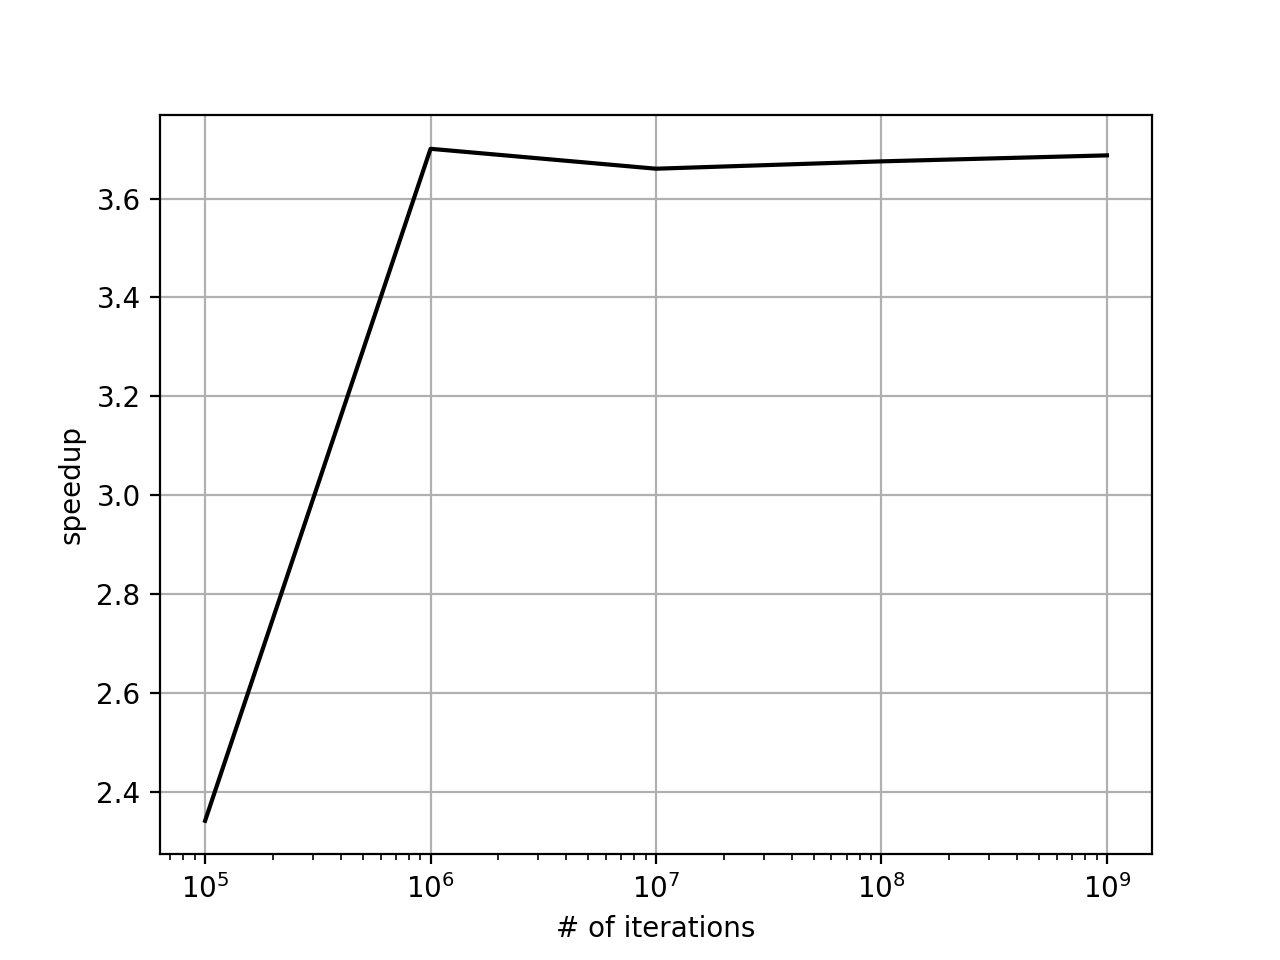
\includegraphics[width=0.8\textwidth]{plots/q1p1.png}
        \caption{speedup vs number of iterations}
        \label{fig:q1p1}
    \end{figure}
    \begin{figure}[H]
        \centering
        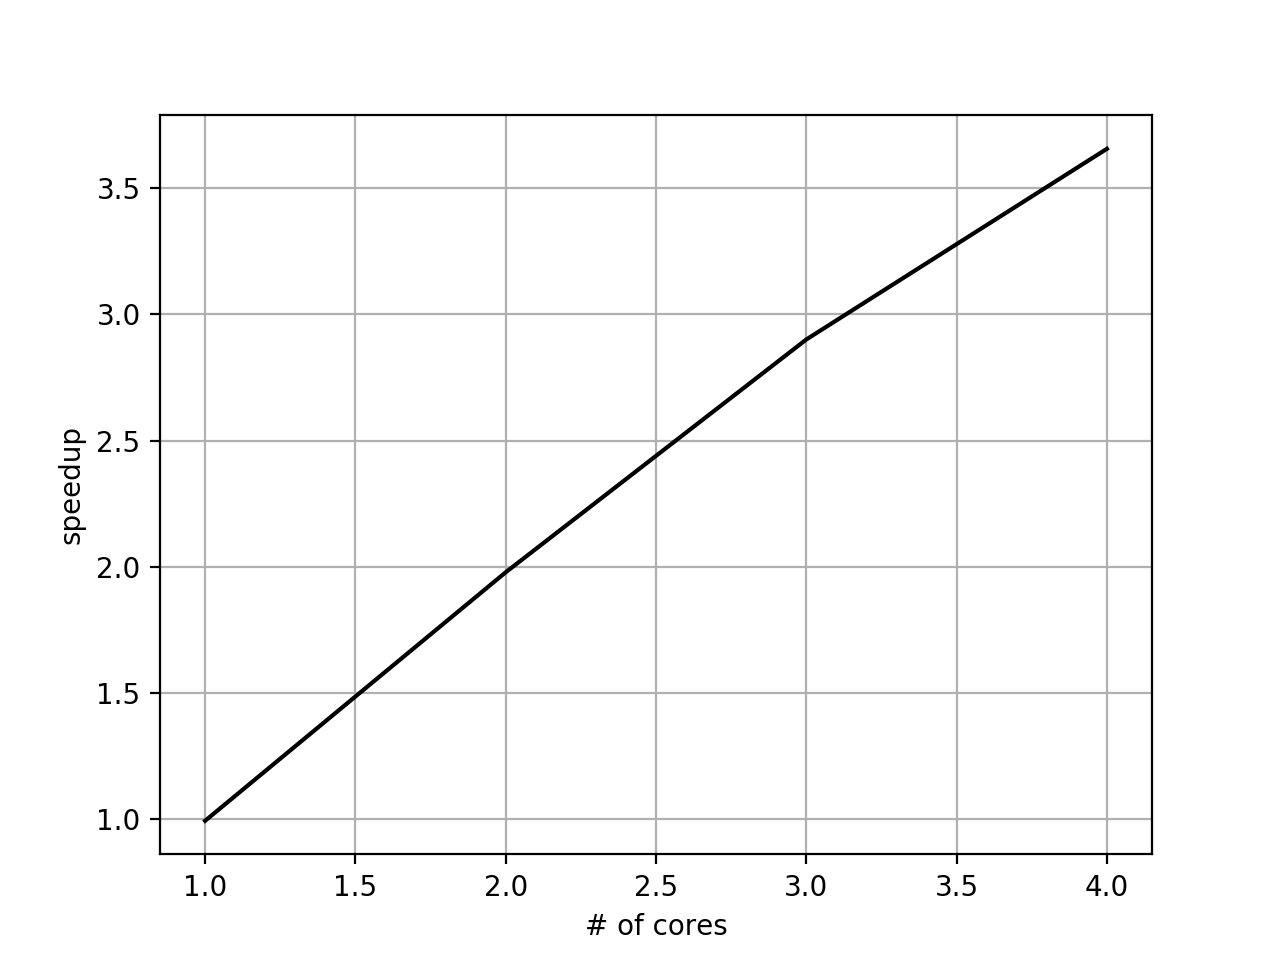
\includegraphics[width=0.8\textwidth]{plots/q1p2.png}
        \caption{speedup vs number of cores}
        \label{fig:q1p2}
    \end{figure}
    
    The above plots show speedup as a function of number of iterations (the problem size) and the number of cores respectively. As the computing unit used during the experiment had 4 cores, the problem could be broken down into 4 parallel processes each having an equal problem size. Hence roughly the speedup should have been at most 4. This is in agreement to our observations which give us a maximum speedup of 3.73.
    
    In \textbf{figure \ref{fig:q1p2}} we see speedup increasing as the number of cores increase. This is in agreement with \textbf{Amdahl's law} which gives us a rough upper limit on speedup in terms of parallelization and also gives us speedup as a function of ratio of the parallel code to serial code and the number of cores in a machine.
    For a piece of code having a ratio $s$ as the serial part and $p$ as a parallel part running on a machine having $n$ cores, the maximum theoretical speedup which can be received is given by :
    
    \begin{equation}
        speedup = \frac{1}{s + \frac{p}{n}}
    \end{equation}
    
    From \textbf{figure \ref{fig:q1p1}} we see the benefits of parallelization for large input sizes. For small input sizes of the order $10^5$ the parallel code is about 2.4 times faster than its serial counterpart. When the input size grows to $10^7$, the speedup increases by nearly 50\%.
    
    \section{Coding strategies}
    \textbf{
        Implement some of the important optimization strategies discussed during the lecture today and measure difference in improvement while using the best strategy.
    }
    \begin{enumerate}
        \item \textbf{Case A}
            \begin{lstlisting}
                for (int i = 0; i < N ; i ++)
                    if( A [ i ] > 100) {
                        flag = true ;
                        break ;
                    }
            \end{lstlisting}
            \textbf{Case B}
            \begin{lstlisting}
                for (int i = 0; i < N ; i ++)
                    if( A [ i ] > 100) {
                        flag = true ;
                    }
            \end{lstlisting}
        \textbf{Observation:} When N = $1 \times 10^9$ in the above cases, and we search in an already instantiated array, the flag is turned true when the value of A[i] is greater than 100 which in this case was kept at i = 500000000. Theoretically, case B does all the iterations while case A has a break condition if the if condition returns true. Case A takes 0.989066 seconds while case B takes 1.956732 seconds.
        
        \parskip 1em
        \textbf{Optimization strategy:} \emph{Trying to perform the least number of operations if the output remains same.}
        \newpage
        \item \textbf{Case A}
            \begin{lstlisting}
                A = B**2.0;
            \end{lstlisting}
            \textbf{Case B}
            \begin{lstlisting}
                A = B*B
            \end{lstlisting}
        \textbf{Observation:} For large floating point numbers of the order $1 \times 10^{25}$, Case A takes 0.000019 seconds while case B takes 0.000000000001 seconds.
        
        \parskip 1em
        \textbf{Optimization strategy:} \emph{Try and avoid more resource consuming operations. In the first case, power does multiplication O(log(n)) times while in the second case, multiplication is done only one time.}
      \item \textbf{Case A}
            \begin{lstlisting}
                int s = 1 , r =2;
                for (int i = 0; i < N ; i ++) {
                    A [ i ] = A [ i ] + s + r * sin (0.523598776) ;
                }
            \end{lstlisting}
            \textbf{Case B}
            \begin{lstlisting}
                int s = 1 , r =2;
                double tmp = s + r * sin (0.523598776) ;
                for (int i = 0; i < N ; i ++) {
                    A [ i ] = A [ i ] + tmp ;
                }
            \end{lstlisting}
        \textbf{Observation:} As we can see in the code, the operation $s + r ∗ sin(x)$ takes place $10^8$ times in case A while it takes place only once in case B which makes it faster. Case A takes 3.584542 seconds, Case B takes 2.890220 seconds.
        
        \parskip 1em
        \textbf{Optimization strategy:} \emph{Reduce the number of registers used to store data, the number of comparisons made or the number of redundant operations}
        \item \textbf{Case A}
            \begin{lstlisting}
                Branched matrix multiplication where N = 1x10000
            \end{lstlisting}
            \textbf{Case B}
            \begin{lstlisting}
                Unbranched matrix multiplication where N = 1x10000
            \end{lstlisting}
        \textbf{Observation:} Case A takes 0.401576 seconds while case B takes 0.194602 seconds. The chances of a branch miss is higher in A then in B because of more number of branches in A than in B. This increases the latency and hence takes more time.
        
        \parskip 1em
        \textbf{Optimization strategy:} \emph{Avoid branching wherever possible.}
    \end{enumerate}
\end{document}